% Please use the skeleton file you have received in the 
% invitation-to-submit email, where your data are already
% filled in. Otherwise please make sure you insert your 
% data according to the instructions in PoSauthmanual.pdf
\documentclass{PoS}
\usepackage{epstopdf}
\usepackage{amsmath,amssymb,amsfonts,amsbsy}
\usepackage{graphicx}
\usepackage[d]{esvect}
\usepackage{calc}

\newcommand{\missET}{\vv{\not{\!\!E}}_T}

\title{Transverse single-spin asymmetries in $W^{\pm}$ and $Z^{0}$ bosons production in p+p collisions at RHIC}

\ShortTitle{$A_{N}$ for $W^{\pm}/Z^{0}$ boson production at RHIC}

\author{\speaker{Salvatore Fazio} and Dmitri Smirnov, for the STAR Collaboration \\ % \thanks{On behalf of the STAR Collaboration.}\\
        Brookhaven National Laboratory\\
        E-mail: \email{sfazio@bnl.gov} \\
        E-mail: \email{dsmirnov@bnl.gov}}

%\author{Dmitri Smirnov\\
%        Brookhaven National Laboratory\\
%        E-mail: \email{dsmirnov@bnl.gov}}

\abstract{The Sivers function $f^{\perp}_{1T}$ describes the correlation of parton transverse momentum with the transverse spin of the nucleon. There is evidence of a quark Sivers effect in semi-inclusive DIS measurements. 
In SIDIS, the quark Sivers function is associated with a final state effect from the gluon exchange between the struck quark and the target nucleon remnants. On the other hand, for the virtual photon production in the Drell-Yan process, the Sivers asymmetry appears as an initial state interaction effect.
As a consequence, the quark Sivers functions are of opposite sign in SIDIS and in Drell-Yan and this non-universality is a fundamental prediction from the gauge invariance of QCD. The experimental test of this sign change is one of the open questions in hadronic physics, and can provide a direct verification of TMD factorization. While luminosities required for a precise measurement of asymmetries in Drell-Yan production are challenging, $W^{\pm}/Z^{0}$ production is equally sensitive to the predicted  sign change and can be well measured  at the STAR experiment. The results can also provide essential input to study the evolution effects of the Sivers function, because of the high $Q^{2}$ in $W/Z^{0}$-production. Here we present the first preliminary measurement of the transverse single spin asymmetry, $A_{N}$, of the $W^{\pm}/Z^{0}$ bosons from the STAR experiment at RHIC. The $W$ boson kinematics are fully reconstructed from the decay lepton and the recoil, by employing a MC-based correction, thus avoiding the dilution that an asymmetry  reconstructed from the decay lepton only would suffer.
}

\FullConference{XXII. International Workshop on Deep-Inelastic Scattering and Related Subjects,\\
		28 April - 2 May 2014\\
		Warsaw, Poland}


\begin{document}

\section{Introduction}
Transversely polarized spin effects have been an extremely active topic among experiment and theory in the past years, because of their connection to transverse momentum dependent (TMD) distributions (leading to a multi-dimensional picture of the proton) and a possible test of the framework and the underlying theory of perturbative QCD. For a quantitative application of the TMD framework to transverse single-spin asymmetries measured in proton-proton collisions, the required two scales (typically $Q^{2}$ and $p_{T}$) are not well defined, excepted for Drell-Yan di-lepton (DY) and $W^{\pm}$,$Z^{0}$ boson production. DY production has been at the center of attention for the non-universality test of the so-called Sivers TMD function, %it requires large integrated luminosities and efficient background reduction. The high mass of $W$-bosons naturally provides a hard $Q^{2}$ scale already and their transverse asymmetries can be directly applied to a global TMD analysis.
$f^{\perp}_{1T}$, which describes the correlation of parton transverse momentum with the transverse spin of the nucleon.  There is evidence of a quark Sivers effect in semi-inclusive DIS (SIDIS) measurements where the quark Sivers function is associated with a final state effect from the gluon exchange between the struck quark and the target nucleon remnants. On the other hand, for the virtual photon production in the Drell-Yan process, the Sivers asymmetry appears in the initial state of the interaction. As a consequence, the quark Sivers functions are of opposite sign in SIDIS and in Drell-Yan
%
\begin{equation}
f^\text{SIDIS}_{q/h^\uparrow} (x, k_\perp) = - f^\text{DY}_{q/h^\uparrow} (x, k_\perp),
\end{equation}
 and this non-universality is a fundamental prediction from the gauge invariance of QCD. 
%From the measured asymmetry it is possible to verify theoretical expectations about the sign change of the Sivers function in Drell-Yan and SIDIS interactions:

The experimental test of this sign change is one of the open questions in hadronic physics, and can provide insights on the TMD factorization. While luminosities required for a meaningful measurement of asymmetries in Drell-Yan production are challenging, $W^{\pm}$ and $Z^{0}$ bosons production is equally sensitive to the predicted sign change and can be well measured at the STAR experiment.  The results can also provide essential input to study the new theoretical concept of evolution effects of transverse momentum dependent distribution functions, because of the high $Q^{2}$ in the $W\rightarrow e \nu$ production due to the large boson mass. The STAR experiment at RHIC is currently the only place in the world where these effects can be tested.

The transverse single spin asymmetry, $A_N$, 
%measured using the lepton decay has been derived~\cite{Kang:2009bp} and the asymmetry 
solely calculated from the lepton decay is predicted to be diluted~\cite{Kang:2009bp}, thus a full reconstruction of the produced boson kinematics is crucial for a meaningful measurement.
Based on the transversely polarized data sample collected in the year 2011 at the c.o.m energy of 500 GeV ($L_{int} = 25$ pb$^{-1}$), an analysis has been performed at STAR to fully reconstruct the $W^{\pm}$ bosons from the lepton decay and all other particles in the recoil from the initial hard scattering. This analysis also includes a first look at $A_{N}$ in $Z^{0}$ production. A proposed measurement with increased statistics in 2016 will be directly competitive with a Drell-Yan measurement in pion-proton scattering at CERN.


\section{The $W^{\pm}$ selection and asymmetry measurement}
A data sample characterized by the $W$ signature has been selected, mostly requiring an isolated high $P_{T} > 25$~GeV electron and a total recoil $P_{T} >18$~GeV.
In order to fully reconstruct the $W$ kinematics the momenta of all $W$ decay
products must be measured. The momentum of the neutrino produced in the leptonically decayed $W$
cannot be measured and can only be indirectly deduced from conservation of the total momentum. 
in the $W$ events produced at $\sqrt{s}=500$~GeV
at STAR we can assume that most of the missing energy, $\missET$ is carried by the neutrino from the
$W$ decay. The assumption ${P}_{\nu, T} \approx \missET$ is based on the
fact that only very little energy is left for anything other than $W$ production
from the primary hard scattering.
In the transverse plane the initial momentum of the system of interacting partons is negligible
and so must be the vector sum of all final particles momenta. We define the
missing transverse energy as a vector restoring the balance in the event:

\begin{equation}
\missET = - \sum_{i \in \parbox[t]{\widthof{\tiny clusters}}{\tiny tracks, clusters}} \vv P_{i,T}.
%miss ET = - \sum_{clusters}{jets, tracks, clusters} P_{i,T}.
\end{equation}

In a typical collider detector like STAR the problem with measuring the missing momentum from the hadronic recoil
is that particles with very high rapidities escape the detector. At the same time, the beam remnants with high
longitudinal momentum carry away only a little portion of the total transverse
momentum. We accounted for the non measured tracks and clusters by using an event-by-event Monte Carlo 
correction to the data.
Knowing its transverse momentum, the longitudinal component of the neutrino's momentum can be reconstructed solving the quadratic equation for the invariant mass of the produced boson

\begin{equation}
\label{eq_InvMass}
M^{2}_{W}=(E_{e}+E_{\nu})^{2} - (\vv P_{e}+\vv P_{\nu})^{2},
\end{equation}
where we assumed the nominal value of the $W$-mass.  Eq.~\ref{eq_InvMass} leads to two possible solutions for $P_{L}^{\nu}$, we chose the smaller one in magnitude because a Monte Carlo study shows that it leads to a much smaller fraction of mis-reconstructed events in our kinematic domain.

Background sources coming from $W^{\pm}\rightarrow \tau^{\pm} \nu_{\tau}$, $Z^{0} \rightarrow e^{+}e^{-}$ and QCD events have been estimated to be contained within maximum a few percent of the selected sample.

%For the $A_{N}$ measurement we are interested in the interaction
%$p^{\uparrow/\downarrow} p \to W^\pm \to e^\pm \nu_e$ in which the spin direction of one
%of the protons is irrelevant, \textit{i.e} unpolarized protons. 
In measuring $A_{N}$ we assume that the beam polarization vector does not significantly
deviate from the vertical direction given by the normal unit vector $\vec n$
along the vertical $y$ axis, $P \equiv \vec{P} \cdot \vec{n}$. 
We also assume the same magnitude of the polarization vector for
spin-up and spin-down bunches, \textit{i.e.} $P = P_\uparrow = P_\downarrow$.
%For unpolarized cross section $\sigma_0 \equiv (\sigma_\uparrow + \sigma_\downarrow)/2$ 
The single spin asymmetry $A_N$ is expressed as:

\begin{align}
\label{eq_anapower}
A_N &= \frac{\sigma_\uparrow - \sigma_\downarrow}{\sigma_\uparrow +
   \sigma_\downarrow}.
\end{align}

We bin our data sample in three observable variables, $\{y, \phi, P_T\}$, of the produced boson. Thus, 
we calculated $A_{N}$ using the square root formula~\cite{sqrtFormula}, which helps to cancel out unwanted effects due to geometry and luminosity.

\begin{align}
A_{N } sin(\phi)= \frac{1}{<P>}
\frac{\sqrt{N_\uparrow(\phi_i)N_\downarrow(\phi_i+\pi)} - \sqrt{N_\uparrow(\phi_i+\pi)N_\downarrow(\phi_i)} } 
{\sqrt{N_\uparrow(\phi_i)N_\downarrow(\phi_i+\pi)} + \sqrt{N_\uparrow(\phi_i+\pi)N_\downarrow(\phi_i)}},
\end{align}
where $N$ is the number of recorded events in the $i-th$ bin with a certain spin ($\uparrow \downarrow$) configuration in the ``left'' ($\phi_{i}$) or in the ``right'' ($\phi_{i} + \pi$) side of the detector and $<P>\simeq 53\%$ is the average RHIC beam polarization for 2011 transverse p+p run.  
For the asymmetry measurement the polarization of one of the beams is ignored by combining the
yields with opposite spins, \textit{e.g.}

\begin{align}
N_{\uparrow}   \equiv N_{\uparrow0}   &= N_{\uparrow\uparrow}   + R_{\frac{0\uparrow}{0\downarrow}} N_{\uparrow\downarrow},\\
N_{\downarrow} \equiv N_{\downarrow0} &= N_{\downarrow\uparrow} + R_{\frac{0\uparrow}{0\downarrow}} N_{\downarrow\downarrow},
\end{align}

\noindent
where re-weighting factor $R_{\frac{0\uparrow}{0\downarrow}}$ addresses a
possible relative difference in the spin-up and spin-down intensities of the
other beam. Studies have shown that $R_{\frac{0\uparrow}{0\downarrow}} \approx
1$ with good precision.

%The spacial distributions of the physical asymmetry and the cross sections are
%the same for the spin-up and spin-down interactions with respect to the spin
%direction. We can use this fact to easily get rid of the  quantities of no
%interest in \eqref{eq:yield}. This is achieved by constructing geometric
%means $\sqrt{N_\uparrow(\phi_i)N_\downarrow(\phi_i+\pi)}$ and
%$\sqrt{N_\uparrow(\phi_i+\pi)N_\downarrow(\phi_i)}$ of the yields

The STAR preliminary results for the $A_{N}$ measurement of the $W^{+}$ and $W^{-}$ bosons production are shown separately in fig.~\ref{Fig:W-An} as a function of $y^{W}$ and $P_{T}^{W}$. 
The systematic uncertainties have been evaluated via e Monte Carlo challenge using a theoretical prediction for the asymmetry from~\cite{Kang:2014} and are added in quadrature.


\begin{figure}[htbp]
  \centering
  \includegraphics[width=0.49\textwidth]{hd_Wp_AsymAmpSqrtVsRap.eps}
  \includegraphics[width=0.49\textwidth]{hd_Wm_AsymAmpSqrtVsRap.eps}
  \includegraphics[width=0.49\textwidth]{hd_Wp_AsymAmpSqrtVsPt.eps}
  \includegraphics[width=0.49\textwidth]{hd_Wm_AsymAmpSqrtVsPt.eps}
  \includegraphics[width=0.44\textwidth]{hd_Z0_AsymAmpSqrtVsRap}
  \caption{Transverse single spin asymmetry amplitude for $W^{\pm}$ and $Z^{0}$ boson production measured at STAR in a pilot run at $\sqrt{s}=500$~GeV with a recorded luminosity of 25~$\text{pb}^{-1}$.}
  \label{Fig:W-An}
\end{figure}


\section{The $Z^{0}$ selection and asymmetry measurement}
The $Z^{0}\rightarrow e^{+}e^{-}$ process has many advantages: it is experimentally very clean and the boson kinematics are easy to reconstruct (thus it carries only the overall systematics coming from the polarization measurement), it is back-ground free and the asymmetry is expected of the same size of the $W^{\pm}$ one. The only big disadvantage is the much lower cross section which makes the measurement very eager of statistics. 

A data sample characterized by the $Z^{0}$ signature has been selected, requiring two isolated high $P_{T} > 25$~GeV electrons, of opposite charge and with an invariant mass within $\pm 20 \%$ of the nominal value.

The STAR preliminary result for the $A_{N}$ measurement of the $Z^{0}$ boson production in a single $y^{Z}$, $P_{T}^{Z}$ bin is shown in fig.~\ref{Fig:W-An}. 


\section{Outlook}
This preliminary study shows that STAR is able to measure the transverse single spin asymmetries $A_{N}$ for fully reconstructed $W^{\pm}$, $Z^{0}$ bosons based on a pilot run of transverse polarized p+p collisions at $\sqrt{s}=500$~GeV with a recorded integrated luminosity of $25~\text{pb}^{-1}$. 
The preliminary results from fig.~\ref{Fig:W-An} can be compared with the most up-to-date theoretical $A_{N}$ predictions for $W^{\pm}$, $Z^{0}$ boson production including TMD-evolution from reference~\cite{Kang:2014}, shown in fig.~\ref{Fig:Run16Proj}.
The production of $W^{\pm}$ bosons at $\sqrt{s}=500$~GeV can lead to the first experimental test of the sign change of the Severs function. Furthermore, it provides an ideal tool to study the spin-flavor structure of sea quarks inside the proton. The left-handed $W$ boson only couples to (anti)quarks of a certain helicity, giving rise to large parity-violating single spin asymmetries. In addition, the coupling of the $W$s to the weak charge correlates directly to quark flavor. Ignoring quark mixing, $W^{\pm}$ bosons are produced through $u+\bar d (d + \bar u)$ interactions. A measurement of the transverse single spin asymmetry will provide the world wide first constraint on the sea quark Sivers function in a x-range, where the measured asymmetry in the  $\bar u$ and $\bar d$ unpolarized sea quark distribution functions, as measured by E866~\cite{E866}, can only be explained by strong non-pQCD contributions. Figure~\ref{Fig:Run16Proj} shows the projected uncertainties for transverse single spin asymmetries of $W^{\pm}$, $Z^{0}$ bosons as function of rapidity and $P_{T}$ for a delivered integrated luminosity of 900 $\text{pb}^{-1}$ compared to 400 $\text{pb}^{-1}$  and an average beam polarization of 50\%. RHIC is capable of delivering 900 $\text{pb}^{-1}$ in 14 weeks running using a dynamic $\beta$* squeeze through the fill. The dynamic $\beta$* squeeze provides a factor 2 increase of the luminosity in a fill as the luminosity profile through the fill is kept flat.

STAR is capability to measure $A_{N}$ for direct photons, for $W^{\pm}$ and $Z^{0}$ bosons, and possibly for DY will provide the world-wide unique opportunity to simultaneously test TMD evolution, access the Sivers function for sea quarks, and test the predicted sign-change for the Sivers function.

\begin{figure}[htbp]
  \centering
  \includegraphics[width=0.32\textwidth]{w_plus.eps}
  \includegraphics[width=0.32\textwidth]{w_minus.eps}
  \includegraphics[width=0.32\textwidth]{z0.eps}
  \caption{Theoretical prediction of $A_{N}$ for $W^{\pm}$ and $Z^{0}$ boson production in p+p collisions at $\sqrt{s}=500$~GeV including TMD-evolution~\cite{Kang:2014}.}
  \label{Fig:An-prediction}
\end{figure}

\begin{figure}[htbp]
  \centering
  \includegraphics[width=0.32\textwidth]{hd_WAsym2016ProjPt_zoom.eps}
  \includegraphics[width=0.32\textwidth]{hd_WAsym2016ProjRap_zoom.eps}
  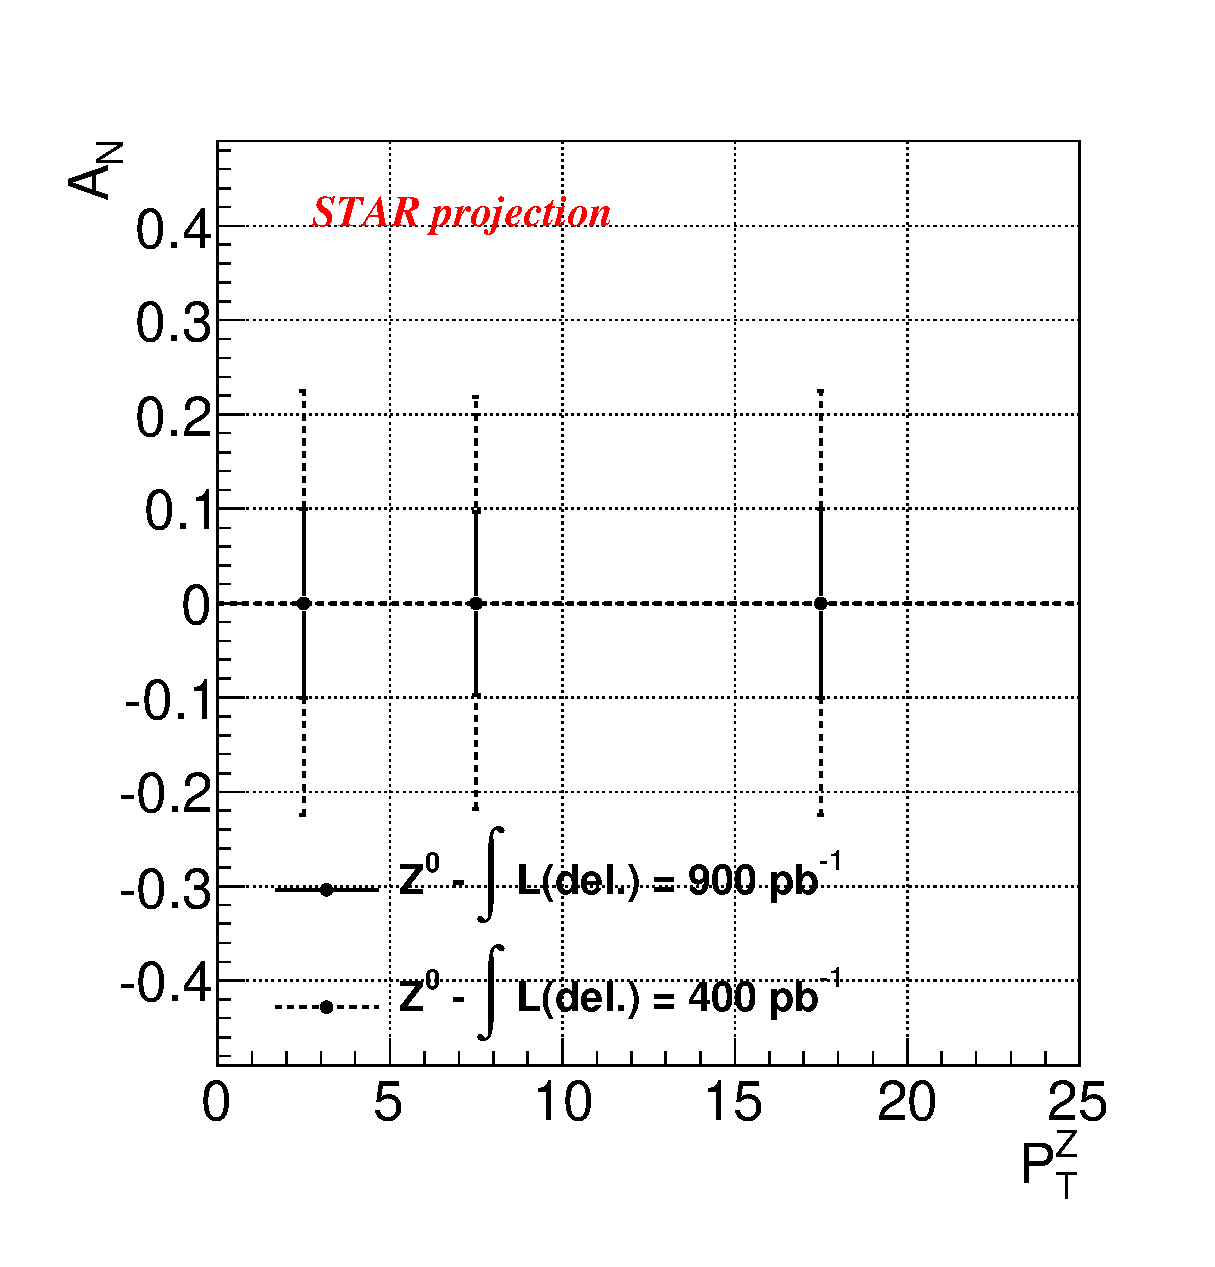
\includegraphics[width=0.32\textwidth]{hd_Z0Asym2016ProjPt.eps}
  \caption{Projections of statistical uncertainties of an $A_{N}$ measurement for  $W^{\pm}$ and $Z^{0}$ boson production at STAR assuming a delivered luminosity of 900~$\text{pb}^{-1}$, the 400~$\text{pb}^{-1}$ case is also shown for comparison.}
  \label{Fig:Run16Proj}
\end{figure}

\begin{thebibliography}{99}

\bibitem{Kang:2009bp} 
  Z.-B.~Kang and J.~-W.~Qiu,
  {\it Phys. Rev. Lett.}  {\bf 103}, 172001 (2009)

\bibitem{sqrtFormula}
B\"{u}ltmann S et al. {\it Phys. Lett. B} {\bf 632} 167 (2006)\\
B\"{u}ltmann S et al. {\it Phys. Lett. B} {\bf 647} 98 (2007)\\
Ohlsen G G and Keaton Jr P W 1973 {\it Nucl. Instr. Meth.} {\bf 109} 41

\bibitem{Kang:2014}
M.~G.~Echevarria, A.~Idilbi, Z.-B.~Kang, I.~Vitev,
{\it Phys. Rev. D} {\bf 89}, 074013 (2014)

\bibitem{E866}
E.A. Hawker et al. {\it Phys. Rev. Lett.} {\bf 80}, 3715 (1998)

\end{thebibliography}

\end{document}


